\chapter{Hình học của không gian đồng nhất}

\lectureoverview{Độ phẳng là một xấp xỉ rất tốt cho vũ trụ quan sát được, nhưng nó không phải là một nguyên lý. Nếu giữ tính đồng nhất và đẳng hướng đồng thời cho phép có độ cong, thì xuất hiện ba kiểu hình học không gian đơn liên: không gian Euclid, không gian cầu và không gian hyperbolic. Metric của chúng có thể được dựng từ cách các lớp vỏ đồng tâm lớn lên theo khoảng cách, và độ cong của chúng có thể được kiểm tra thông qua kích thước góc và số lượng vật thể. Không gian phẳng cũng có thể là hữu hạn khi topo của nó là hình xuyến. Cuối cùng, gắn một thừa số tỉ lệ phụ thuộc thời gian vào bất kỳ không gian đồng nhất nào trong số này sẽ cho các metric không-thời gian vũ trụ học và định luật Hubble; động lực học của thừa số tỉ lệ đó phải xuất phát từ thuyết tương đối rộng.}

\section{Độ phẳng là một quan sát, không phải một nguyên lý}

Cho đến nay chúng ta đã xem không gian là phẳng và hầu như chưa nói gì về hình học không-thời gian. Quan sát biện minh cho không gian phẳng như một xấp xỉ rất tốt, nhưng không nâng độ phẳng lên thành một định luật. Điều mà các phép đo thực sự cho ta biết là mọi bán kính cong đều phải lớn so với vùng mà chúng ta đã khảo sát. Không gian có thể phẳng đúng hẳn, cong dương, hoặc cong âm. Trên những thang đo vượt xa vùng quan sát được, chúng ta vẫn chưa biết mô tả nào là đúng.

Vì vậy, chúng ta nới lỏng một giả thiết trong khi vẫn giữ giả thiết kia. Chúng ta sẽ không giả sử độ phẳng, nhưng sẽ tiếp tục giả sử rằng không gian là đồng nhất và đẳng hướng. Đây là một giả thuyết làm việc, không phải một tín điều. Để tìm hiểu các hệ quả của nó, ta giả sử nó rồi tính toán; sau đó ta có thể từ bỏ nó và hỏi xem một vũ trụ không đồng nhất sẽ hành xử khác đi ra sao.

Đồng nhất nghĩa là mọi điểm đều có cùng đặc tính hình học. Một người quan sát di chuyển đến nơi khác và lặp lại các thí nghiệm hình học cục bộ sẽ thu được cùng kết quả. Đẳng hướng nghĩa là không có hướng nào được ưu tiên. Những điều kiện này loại trừ hầu như mọi mặt cong mà ta thường nghĩ đến đầu tiên. Một paraboloid cong mạnh hơn gần đỉnh của nó so với ở xa. Một ellipsoid thuôn dài khác nhau ở các cực và ở phần eo. Một mặt cầu lồi lõm, hoặc bề mặt Trái Đất khi phân giải được núi và thung lũng, thì cong nhưng không đồng nhất. Câu hỏi của vũ trụ học hẹp hơn:
\begin{quote}
Những không gian nào có thể cong mà vẫn có vẻ giống hệt nhau về mặt hình học từ mọi điểm và theo mọi hướng?
\end{quote}

Tạm thời bỏ qua các phép đồng nhất toàn cục, có ba đáp án có độ cong hằng: không gian phẳng, không gian cầu cong dương và không gian hyperbolic cong âm. Sự bảo lưu về các phép đồng nhất toàn cục này là quan trọng; về sau chúng ta sẽ dựng một hình xuyến phẳng hữu hạn và sửa lại phát biểu quá đơn giản rằng ba trường hợp ấy bao quát mọi khả năng.

\section{Metric và tọa độ của người quan sát}

Trước hết chúng ta chỉ bàn về không gian, không phải không-thời gian. Hình học của nó được mã hóa trong một metric: một quy tắc cho bình phương khoảng cách \(ds^2\) giữa các điểm lân cận. Một khi quy tắc cục bộ đó đã được biết ở mọi nơi, các độ dài, góc, diện tích, thể tích, các đường trắc địa và độ cong đều có thể được khôi phục từ nó.

Đối với mặt phẳng Euclid và không gian Euclid ba chiều, tọa độ Descartes cho
\begin{equation}
ds_2^2=dx^2+dy^2,
\qquad
ds_3^2=dx^2+dy^2+dz^2.
\label{eq:c03-cartesian-flat}
\end{equation}
Việc thêm chiều thứ ba chỉ đơn giản là thêm hạng trực giao \(dz^2\), nhưng điểm quan trọng không phải là sự đơn giản của công thức này. Mà là phương trình~\eqref{eq:c03-cartesian-flat} xác định hoàn toàn hình học cục bộ.

\begin{figure}[htbp]
\centering
\includegraphics[width=0.74\textwidth]{lecture_03_figure_02.png}
\caption{Metric Descartes của không gian phẳng ba chiều, như được viết trên bảng.}
\label{fig:c03-cartesian-board}
\lectureframe{00:05:13.138}
\end{figure}

Tọa độ Descartes che khuất cách một nhà thiên văn tiếp cận vũ trụ. Chúng ta chiếm một điểm, nhìn ra ngoài theo hướng, và sắp xếp những gì ta thấy theo góc và khoảng cách. Trong một vũ trụ hai chiều, trường nhìn theo nghĩa đen sẽ là một vòng tròn các hướng quanh ta. Vì thế, tọa độ cực không chỉ thanh nhã; chúng làm lộ ra hình học góc mà vũ trụ học sử dụng.

Gọi \(r\) là khoảng cách xuyên tâm và \(\theta\) là hướng. Mặt phẳng Euclid ấy nay có metric
\begin{equation}
ds^2 = dr^2 + r^2 d\theta^2.
\label{eq:c03-polar-flat}
\end{equation}
Với một góc nhỏ cố định \(d\theta\), độ tách ngang là \(r\,d\theta\). Nó tăng tuyến tính khi ta đi ra xa, nên đóng góp bình phương của nó vào metric vì thế là \(r^2d\theta^2\).

Hạng góc bản thân nó là metric của một không gian một chiều. Một đường tròn là một 1-cầu, ký hiệu \(S^1\), và metric của đường tròn đơn vị theo quy ước được viết
\begin{equation}
d\Omega_1^2 = d\theta^2,
\qquad\text{so that}\qquad
ds^2 = dr^2 + r^2 d\Omega_1^2.
\label{eq:c03-omega-one}
\end{equation}
Trên bảng dùng \(d\Omega^2\) mà không có chỉ số dưới đọc được; phần định nghĩa bằng lời xác định đối tượng được ngụ ý là \(d\Omega_1^2\).

\begin{figure}[htbp]
\centering
\includegraphics[width=0.74\textwidth]{lecture_03_figure_03.png}
\caption{Hình phác thảo theo tọa độ cực và metric của không gian phẳng. Trên bảng hiện \(d\Omega^2\); lời giải thích cho biết đó là metric của đường tròn đơn vị \(d\Omega_1^2=d\theta^2\).}
\label{fig:c03-polar-board}
\lectureframe{00:08:37.254}
\end{figure}

\begin{figure}[htbp]
\centering
\begin{tikzpicture}[scale=1.2]
\draw[->] (-1.2,0)--(1.8,0);
\draw[->] (0,-1.2)--(0,1.8);
\draw[thick] (0,0)--(1.3,1.1);
\draw (0.7,0.7) node[above] {$r$};
\draw (0.58,0) arc (0:40:0.58);
\draw (0.8,0.22) node {$\theta$};
\end{tikzpicture}
\caption{Bản dựng lại rõ ràng của hệ tọa độ cực lấy người quan sát làm tâm được dùng trong phương trình~\eqref{eq:c03-omega-one}.}
\label{fig:c03-polar-redraw}
\end{figure}

\begin{classroomqa}
\audiencequestion{Liệu \(d\theta^2\) có thực sự đo khoảng cách dọc theo chu vi không?}
\lecturerresponse{Có. Trên đường tròn đơn vị, độ dài cung bằng góc tính theo radian, nên các điểm lân cận cách nhau bởi \(d\theta\) có độ tách nội tại bình phương là \(d\theta^2\). Đường tròn có chu vi \(2\pi\), và tích phân \(ds=d\theta\) một vòng quanh nó cho đúng \(2\pi\). Nhân với \(r^2\) sẽ phóng đường tròn đơn vị thành đường tròn bán kính \(r\) trong mặt phẳng. \lecturetimestamp{00:09:11--00:09:26}}
\end{classroomqa}

Từ \emph{nội tại} là thiết yếu. Nếu ta nhúng đường tròn đơn vị vào một mặt phẳng Euclid, ta có thể mô tả nó bằng
\begin{equation}
x^2 + y^2 = 1.
\end{equation}
Phương trình đó mô tả cách đường tròn nằm trong một không gian lớn hơn. Nó không cần thiết đối với một cư dân chỉ có thể đo các khoảng cách dọc theo đường tròn. Ta có thể uốn một sợi cáp quang mềm thành một vòng kín méo lệch mà không kéo dãn nó. Dáng vẻ của nó trong mặt phẳng sẽ thay đổi, nhưng chu vi nội tại và metric của nó thì không. Các độ tăng bằng nhau của \(\theta\) vẫn sẽ đánh dấu các khoảng cách bằng nhau dọc theo sợi. Vì thế, hình học phải được tách khỏi hình dạng ngẫu nhiên do một phép nhúng cung cấp.

\begin{figure}[htbp]
\centering
\includegraphics[width=0.64\textwidth]{lecture_03_figure_04.png}
\caption{Trên bảng so sánh một đường tròn đơn vị tròn đều với một vòng kín bị biến dạng. Nếu vòng đó bị uốn mà không bị kéo dãn, cả hai có cùng metric một chiều nội tại.}
\label{fig:c03-intrinsic-board}
\lectureframe{00:10:34.205}
\end{figure}

\begin{figure}[htbp]
\centering
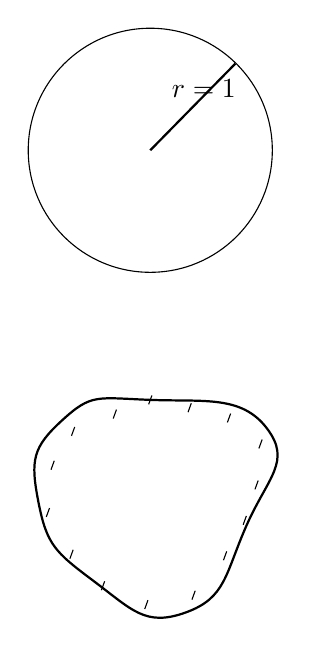
\begin{tikzpicture}[scale=1.0]
\draw (0,0) circle (1.55);
\draw[thick] (0,0)--(1.08,1.1);
\draw (0.68,0.78) node {$r=1$};

\begin{scope}[yshift=-4.35cm]
\draw[thick]
plot[smooth cycle, tension=0.95] coordinates
{(0,1.18) (1.48,0.82) (1.22,-0.42) (0.45,-1.52) (-0.72,-1.12) (-1.42,-0.12) (-1.12,0.92)};
\foreach \p in {(0,1.18),(0.5,1.08),(1.0,0.95),(1.4,0.62),(1.35,0.1),(1.2,-0.35),(0.95,-0.8),(0.55,-1.3),(-0.05,-1.42),(-0.6,-1.18),(-1.0,-0.78),(-1.3,-0.25),(-1.24,0.35),(-0.98,0.78),(-0.45,1.0)}{
\draw[rotate around={70:\p}] \p ++(-0.06,0) -- ++(0.12,0);
}
\end{scope}
\end{tikzpicture}
\caption{Khoảng cách nội tại vẫn được bảo toàn qua một biến dạng ngoại tại: một cư dân một chiều đo được cùng một chu vi trong cả hai phép nhúng.}
\label{fig:c03-intrinsic-redraw}
\end{figure}

Giờ đây không gian phẳng có thể được hiểu như một họ các đường tròn lồng nhau quanh người quan sát. Lớp vỏ ở khoảng cách \(r\) là một bản sao của đường tròn đơn vị được phóng lớn theo \(r\), và đó chính xác là điều mà thừa số \(r^2d\Omega_1^2\) ghi lại.

\section{Độ cong dương: các lớp vỏ khép lại}

Một mặt cầu thì cong nhưng đồng nhất: không điểm nào trên một mặt cầu tròn hoàn hảo được phân biệt về mặt hình học với điểm nào khác. Ta có thể dựng metric của nó mà không cần viện đến một hình ảnh ba chiều bên ngoài. Hãy tưởng tượng các nhà thiên văn hai chiều sống trên một \(2\)-cầu đơn vị và đặt gốc tọa độ tại chính vị trí của họ.

Đường tròn ở khoảng cách trắc địa nhỏ \(r\) quanh họ thì nhỏ. Khi \(r\) tăng, các đường tròn lớn dần, đạt chu vi lớn nhất ở nửa vòng quanh mặt cầu, rồi co lại cho đến khi chúng sụp tại điểm đối cực. Sự lớn lên và co lại này diễn ra theo \emph{khoảng cách}, chứ không theo thời gian. Mặt cầu là tĩnh trong suốt phép dựng này.

Ở đây \(r\) là khoảng cách góc dọc theo mặt cầu đơn vị chứ không phải khoảng cách Euclid tính từ một tâm:
\[
0 \le r \le \pi.
\]
Tại \(r=0\) là gốc đã chọn, tại \(r=\pi/2\) là đường tròn lớn ở nửa vòng quanh, và tại \(r=\pi\) là điểm đối cực. Bán kính của lớp vỏ giờ là \(\sin r\), nên thừa số phẳng \(r^2\) được thay bằng \(\sin^2r\):
\begin{equation}
d\Omega_2^2 = dr^2 + \sin^2 r\, d\Omega_1^2
            = dr^2 + \sin^2 r\, d\theta^2.
\label{eq:c03-two-sphere}
\end{equation}
Các đầu mút và trung điểm cho đúng như yêu cầu:
\begin{equation}
\sin 0=0,
\qquad
\sin\frac{\pi}{2}=1,
\qquad
\sin\pi=0.
\end{equation}
Vì thế, các lớp vỏ bắt đầu với kích thước bằng 0, đạt kích thước cực đại, rồi lại khép kín.

\begin{figure}[htbp]
\centering
\includegraphics[width=0.82\textwidth]{lecture_03_figure_05.png}
\caption{Sự chuyển từ các đường tròn lồng nhau trong không gian phẳng sang các lớp vỏ trên mặt cầu. Công thức phía dưới bị che khuất một phần trong khung hình; phần suy dẫn bằng lời cho ta phép thay \(r^2\mapsto\sin^2r\) trong phương trình~\eqref{eq:c03-two-sphere}.}
\label{fig:c03-spherical-board}
\lectureframe{00:16:11.701}
\end{figure}

\begin{figure}[htbp]
\centering
\resizebox{\linewidth}{!}{%
\begin{tikzpicture}[scale=0.92]
\begin{scope}[xshift=-4.15cm]
\draw[->] (-1.7,0)--(1.9,0);
\draw[->] (0,-1.7)--(0,1.9);
\draw (0,0) circle (0.45);
\draw (0,0) circle (0.9);
\draw (0,0) circle (1.35);
\draw[thick] (0,0)--(1.45,1.2);
\draw (0.56,0.18) arc (18:40:0.63);
\draw (0.94,0.44) node {$\theta$};
\end{scope}

\begin{scope}[xshift=4.15cm]
\draw (0,0) circle (2.0);
\fill (0,-2.0) circle (1.5pt);
\fill (2.0,0) circle (1.5pt);
\fill (0,2.0) circle (1.5pt);
\draw[thick] (0,-2.0) arc (-90:90:2.0);
\draw (0,-2.35) node {$r=0$};
\draw (2.75,0) node {$r=\pi/2$};
\draw (0,2.35) node {$r=\pi$};
\end{scope}
\end{tikzpicture}
}%
\caption{Các lớp vỏ phẳng lớn mãi, còn các lớp vỏ cầu thì lớn đến cực đại tại \(r=\pi/2\) và khép lại tại \(r=\pi\).}
\label{fig:c03-shells-flat-sphere}
\end{figure}

Ký hiệu \(d\Omega_2^2\) chỉ metric của mặt cầu đơn vị \(2\)-chiều, cũng như \(d\Omega_1^2\) chỉ metric của các lớp vỏ tròn của nó. Cùng một cách xây dựng đệ quy ấy cũng áp dụng được khi tăng thêm một chiều. Trong không gian ba chiều phẳng, ở bán kính cố định, lớp vỏ bao quanh ta là một mặt cầu \(2\)-chiều:
\begin{equation}
ds_{\text{flat},3}^2 = dr^2 + r^2 d\Omega_2^2.
\label{eq:c03-flat-three-polar}
\end{equation}
Nếu các lớp vỏ mặt cầu \(2\)-chiều ấy nở ra rồi khép lại theo hệ số \(\sin r\), thì không gian thu được là một mặt cầu đơn vị \(3\)-chiều:
\begin{equation}
d\Omega_3^2 = dr^2 + \sin^2 r\, d\Omega_2^2.
\label{eq:c03-three-sphere}
\end{equation}
Mặt cầu \(3\)-chiều khó hình dung vì phép nhúng quen thuộc của nó sẽ cần bốn chiều Euclid. Tuy nhiên, metric ấy là đầy đủ và không cần hình ảnh nào. Quanh bất kỳ người quan sát nào được chọn đều có các mặt cầu \(2\)-chiều lồng nhau; chúng lớn dần đến cực đại rồi co lại về điểm đối cực.

\begin{classroomqa}
\audiencequestion{Người quan sát có ở tâm của mặt cầu không?}
\lecturerresponse{Người quan sát ở tâm của \emph{các lớp vỏ tọa độ}, chứ không ở một tâm hình học đặc biệt nào. Gốc tọa độ là một điểm trên không gian, và bất kỳ người quan sát nào khác cũng có thể chọn chính điểm của mình làm \(r=0\) và thu được cùng một metric. Tính đồng nhất chính là phát biểu rằng không có lựa chọn nào như vậy được ưu tiên. \lecturetimestamp{00:19:21--00:20:27}}
\end{classroomqa}

Chỉ để trực quan hóa, đường tròn đơn vị và mặt cầu đơn vị \(2\)-chiều có thể được nhúng vào các không gian Euclid:
\begin{equation}
x^2+y^2=1,
\qquad
x^2+y^2+z^2=1.
\end{equation}
Các phương trình này mô tả các phép nhúng, không phải vật lý bổ sung. Một con kiến bị giới hạn trên đường tròn hoặc mặt cầu có thể xác định metric nội tại mà không phát hiện ra không gian Euclid bao quanh. Tương tự, \(S^3\) không phải là một khối cầu thông thường với một biên bí ẩn. Nó là toàn bộ không gian ba chiều được mô tả bởi phương trình~\eqref{eq:c03-three-sphere}.

\section{Độ cong làm thay đổi những gì ta thấy như thế nào}

Hình học chỉ trở thành vật lý khi nó làm thay đổi một quan sát. Giả sử một vật thể có đường kính ngang đã biết \(d\), khoảng cách xuyên tâm của nó \(r\) đã được suy ra độc lập, và kích thước góc của nó \(d\theta\) được đo trên bầu trời. Các thiên hà đem lại một ví dụ trực quan gần đúng; vũ trụ học chính xác hơn sử dụng các thước đo chuẩn và các nến chuẩn đã được hiệu chuẩn. Thông tin về khoảng cách có thể được tổng hợp từ độ lệch đỏ phổ, quan hệ Hubble, độ sáng và sự hiệu chuẩn chéo giữa các loại đối tượng khác nhau.

Trong không gian phẳng, giữ \(r\) không đổi trên bề ngang của vật thể. Phương trình~\eqref{eq:c03-polar-flat} cho
\begin{equation}
d^2 = r^2 d\theta^2.
\label{eq:c03-flat-angle-step}
\end{equation}
Do đó
\begin{equation}
d\theta = \frac{d}{r}.
\label{eq:c03-flat-angle}
\end{equation}
Kích thước góc giảm theo tỉ lệ nghịch với khoảng cách.

Trên một mặt cầu đơn vị, kích thước ngang của lớp vỏ là \(\sin r\) chứ không phải \(r\):
\begin{equation}
d^2 = \sin^2 r\, d\theta^2,
\qquad\text{hence}\qquad
d\theta = \frac{d}{\sin r}.
\label{eq:c03-spherical-angle}
\end{equation}
Với \(0<r<\pi\), ta có \(\sin r<r\), nên cùng một vật thể ở cùng khoảng cách xuyên tâm sẽ trông lớn hơn so với trong không gian phẳng. Kích thước góc của nó ban đầu giảm, đạt cực tiểu tại xích đạo, rồi tăng lên khi lớp vỏ co lại. Trong lý tưởng hóa giới hạn, tại điểm đối cực mọi hướng gặp nhau và ảnh trải khắp bầu trời.

\begin{classroomqa}
\audiencequestion{Đây có phải là cùng ý tưởng được dùng để suy ra độ cong từ bức xạ nền vi sóng vũ trụ không?}
\lecturerresponse{Đúng. Plasma sơ khai cung cấp một thang kích thước vật lý đặc trưng thông qua các dao động âm học của nó. Ta đo góc mà thước đo chuẩn ấy chắn và so sánh với góc được dự đoán bởi từng hình học. Các đối tượng không nhất thiết phải thực sự là các thiên hà; phép so sánh cốt yếu là giữa một thang kích thước ngang đã biết và kích thước góc quan sát được của nó. \lecturetimestamp{00:37:37--00:38:12}}
\end{classroomqa}

Thể tích các vỏ cung cấp một phép kiểm tra thứ hai. Trong không gian phẳng ba chiều, diện tích của một vỏ tỉ lệ với \(r^2\); trên một \(3\)-cầu đơn vị, nó tỉ lệ với \(\sin^2r\). Vì vậy, đối với một quần thể đồng nhất, số lượng vật thể trên một vỏ cầu lúc đầu tăng theo khoảng cách rồi giảm đi sau xích đạo. Độ cong dương dự đoán một dấu hiệu kép so với không gian phẳng: các thước đo chuẩn ở đủ xa trông quá lớn, và các vỏ ở đủ xa chứa quá ít vật thể.

\begin{figure}[htbp]
\centering
\resizebox{\linewidth}{!}{%
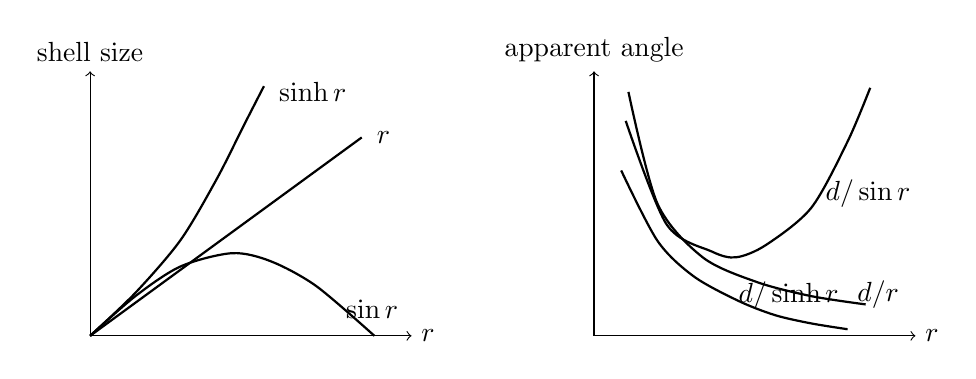
\begin{tikzpicture}[x=1.15cm,y=1.05cm]
\begin{scope}
\draw[->] (0,0)--(3.55,0) node[right] {$r$};
\draw[->] (0,0)--(0,3.2) node[above] {shell size};

\draw[thick] (0,0)--(3.0,2.4);
\draw (3.06,2.4) node[right] {$r$};

\draw[thick]
plot[smooth] coordinates {(0,0) (0.5,0.48) (1.0,0.84) (1.57,1.0) (2.0,0.9) (2.5,0.6) (3.14,0)};
\draw (2.72,0.55) node[below right] {$\sin r$};

\draw[thick]
plot[smooth] coordinates {(0,0) (0.5,0.52) (1.0,1.16) (1.4,1.9) (1.7,2.55) (1.92,3.02)};
\draw (1.98,2.95) node[right] {$\sinh r$};
\end{scope}

\begin{scope}[xshift=6.4cm]
\draw[->] (0,0)--(3.55,0) node[right] {$r$};
\draw[->] (0,0)--(0,3.2) node[above] {apparent angle};

\draw[thick]
plot[smooth] coordinates {(0.38,2.95) (0.7,1.6) (1.2,0.95) (1.8,0.65) (2.4,0.48) (3.0,0.38)};
\draw (2.8,0.5) node[right] {$d/r$};

\draw[thick]
plot[smooth] coordinates {(0.35,2.6) (0.8,1.35) (1.3,1.02) (1.57,0.95) (1.9,1.1) (2.4,1.55) (2.8,2.35) (3.05,3.0)};
\draw (2.45,1.72) node[right] {$d/\sin r$};

\draw[thick]
plot[smooth] coordinates {(0.3,2.0) (0.7,1.15) (1.1,0.72) (1.6,0.42) (2.0,0.25) (2.4,0.15) (2.8,0.08)};
\draw (2.15,0.2) node[above] {$d/\sinh r$};
\end{scope}
\end{tikzpicture}
}%
\caption{Các thừa số vỏ theo bán kính và các quy luật kích thước góc tương ứng. Độ cong dương làm vỏ khép lại; độ cong âm làm nó tăng theo hàm mũ.}
\label{fig:c03-shell-angular-laws}
\end{figure}

\begin{classroomqa}
\audiencequestion{Tọa độ bán kính có trở nên vô hạn khi ta tiếp tục đi quanh mặt cầu không?}
\lecturerresponse{Không. Trên mặt cầu đơn vị, \(r\) là khoảng cách góc trắc địa và chỉ chạy từ \(0\) đến \(\pi\). Tại \(r=\pi\), vỏ đã co sụp tại điểm đối cực. Ở đây ta đang xét một hình học không gian cố định, chứ không theo dõi một vật đi ra xa theo thời gian. Việc đưa vào bán kính độ cong ở phần sau sẽ nhân mọi khoảng cách vật lý với bán kính đó nhưng không làm thay đổi khoảng giá trị vô thứ nguyên này. \lecturetimestamp{00:39:30--00:40:35}}
\end{classroomqa}

\section{Phép chiếu không phải là hình học}

Trước khi chuyển sang độ cong âm, sẽ hữu ích nếu thấy một hình học chuẩn xác có thể bị một hình vẽ làm méo đến mức nào. Đặt một mặt cầu lên một mặt phẳng tiếp xúc với nó tại cực nam. Vẽ một đường thẳng từ cực bắc đi qua mỗi điểm \(P\) trên mặt cầu rồi kéo dài tới mặt phẳng tại \(P'\). Đây là phép chiếu lập thể. Cực bắc được gửi ra vô cực. Một vùng nhỏ gần cực nam được biểu diễn với rất ít méo dạng, trong khi những vùng có kích thước nội tại bằng nhau gần cực bắc lại trở nên khổng lồ trên mặt phẳng.

Sự méo thuộc về bản đồ, không phải về mặt cầu. Mặt cầu ban đầu vẫn đồng nhất dù ảnh phẳng của nó gán các kích thước tọa độ rất khác nhau cho những vùng tương đương. Ta sẽ lại cần sự phân biệt này khi một không gian hyperbolic vô hạn được nén vào một đĩa hữu hạn.

\begin{figure}[htbp]
\centering
\resizebox{\linewidth}{!}{%
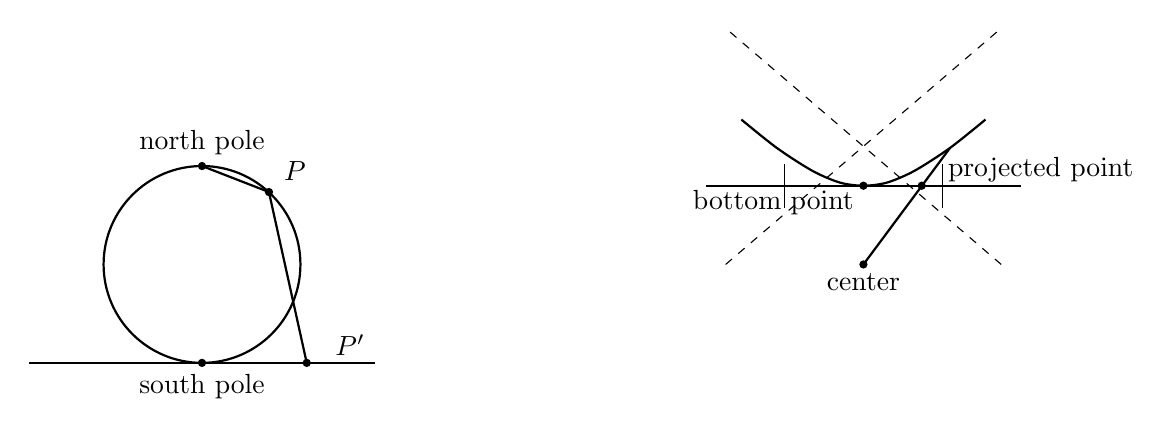
\begin{tikzpicture}[scale=1.0]
\begin{scope}[xshift=-4.2cm]
\draw[thick] (-2.2,-1.25)--(2.2,-1.25);
\draw[thick] (0,0) circle (1.25);
\fill (0,1.25) circle (1.5pt);
\fill (0,-1.25) circle (1.5pt);
\draw (0,1.55) node {north pole};
\draw (0,-1.55) node {south pole};

\fill (0.85,0.92) circle (1.5pt);
\draw (0.92,1.18) node[right] {$P$};
\draw[thick] (0,1.25)--(0.85,0.92)--(1.33,-1.25);
\fill (1.33,-1.25) circle (1.5pt);
\draw (1.57,-1.03) node[right] {$P'$};
\end{scope}

\begin{scope}[xshift=4.2cm]
\draw[thick] (-2.0,1)--(2.0,1);
\draw[dashed] (-1.75,0)--(1.75,3.0);
\draw[dashed] (1.75,0)--(-1.75,3.0);
\draw[thick]
plot[smooth] coordinates
{(-1.55,1.84) (-1.1,1.48) (-0.65,1.19) (-0.3,1.04) (0,1.0) (0.3,1.04) (0.65,1.19) (1.1,1.48) (1.55,1.84)};
\fill (0,0) circle (1.5pt);
\fill (0,1) circle (1.5pt);
\draw (0,-0.22) node {center};
\draw (0,0.78) node[left] {bottom point};
\draw[thick] (0,0)--(1.1,1.48);
\fill (0.74,1.0) circle (1.5pt);
\draw (0.95,1.2) node[right] {projected point};
\draw (-1,0.72) -- (-1,1.28);
\draw (1,0.72) -- (1,1.28);
\end{scope}
\end{tikzpicture}
}%
\caption{Bên trái: phép chiếu lập thể gửi cực bắc của một mặt cầu ra vô cực. Bên phải: một hyperboloid có thể được chiếu vào một đĩa hữu hạn, ở đây được biểu diễn bằng một đoạn cắt ngang. Sự méo tọa độ không phá hủy tính đồng nhất nội tại.}
\label{fig:c03-projections}
\end{figure}

\section{Độ cong âm: Các vỏ tăng nhanh hơn so với không gian phẳng}

Hình học đồng nhất đơn liên thứ ba thay \(\sin r\) bằng hàm sin hyperbol. Các metric đơn vị của nó trong hai và ba chiều là
\begin{equation}
dh_2^2 = dr^2 + \sinh^2 r\, d\Omega_1^2,
\label{eq:c03-hyperbolic-two}
\end{equation}
\begin{equation}
dh_3^2 = dr^2 + \sinh^2 r\, d\Omega_2^2.
\label{eq:c03-hyperbolic-three}
\end{equation}
Tọa độ \(r\) nay chạy trên
\begin{equation}
0\le r<\infty.
\end{equation}
Gần gốc tọa độ, \(\sinh r\approx r\), nên hình học này cục bộ là Euclid. Ở xa, các vỏ của nó tăng nhanh hơn nhiều so với các vỏ Euclid và không bao giờ ngoặt lại.

Quy luật tăng trưởng suy ra từ
\begin{equation}
\sin r = \frac{e^{ir}-e^{-ir}}{2i},
\qquad
\sinh r = \frac{e^r-e^{-r}}{2}.
\label{eq:c03-sin-sinh}
\end{equation}
Khi \(r\) lớn, \(\sinh r\sim e^r/2\). Vì vậy trong hai chiều, chu vi tăng theo hàm mũ theo bán kính; trong ba chiều, diện tích vỏ tăng như \(\sinh^2r\sim e^{2r}/4\). Một phân bố đồng nhất vì thế chứa tương ứng nhiều vật thể trên một vỏ ở xa.

Đối với một vật thể vuông góc với phương nhìn có kích thước \(d\),
\begin{equation}
d^2 = \sinh^2 r\, d\theta^2,
\qquad\text{so}\qquad
d\theta = \frac{d}{\sinh r}.
\label{eq:c03-hyperbolic-angle}
\end{equation}
Khi \(r\) lớn,
\begin{equation}
d\theta \sim 2d\,e^{-r}.
\end{equation}
Vì vậy, độ cong âm cho dấu hiệu ngược với độ cong dương: các thước chuẩn ở xa trông quá nhỏ, còn các lớp vỏ ở xa thì chứa quá nhiều vật thể so với không gian phẳng.

\begin{classroomqa}
\audiencequestion{Các miền giá trị của tọa độ bán kính phân biệt không gian cầu và không gian hyperbol như thế nào?}
\lecturerresponse{Trên mặt cầu đơn vị, \(r\) dừng lại ở điểm đối cực, \(r=\pi\). Trong không gian hyperbol, nó tiếp tục không bị chặn, \(0\le r<\infty\). Thừa số lớp vỏ cho thấy cùng một sự tương phản: \(\sin r\) trở về không, trong khi \(\sinh r\) tăng mãi mãi. \lecturetimestamp{00:52:46--00:53:25}}
\end{classroomqa}

Có một phép nhúng làm cho tính đồng nhất bớt bí ẩn hơn. Đưa vào các tọa độ của không gian bao quanh \(T,x,y\), trong đó \(T\) chỉ là một tọa độ nhúng và \emph{không phải} thời gian vũ trụ học, rồi lấy nhánh trên
\begin{equation}
T^2 - x^2 - y^2 = 1.
\label{eq:c03-hyperboloid}
\end{equation}
Trang bị cho không gian bao quanh mêtric có chữ ký Lorentz
\begin{equation}
d\ell_{\mathrm{emb}}^2=-dT^2+dx^2+dy^2.
\label{eq:c03-ambient-minkowski}
\end{equation}
Mêtric cảm sinh trên hyperboloid là xác định dương. Các phép biến đổi Lorentz bảo toàn cả hai phương trình~\eqref{eq:c03-hyperboloid} và~\eqref{eq:c03-ambient-minkowski}, và chúng có thể đưa bất kỳ điểm nào của nhánh trên tới bất kỳ điểm nào khác. Theo nghĩa đó, việc thay đổi gốc trên không gian hyperbol giống như nghiêng trục thời gian trong không gian bao quanh phụ trợ. Mọi điểm đều tương đương về mặt hình học.

Chiếu hyperboloid vào một đĩa, và các điểm ở xa vô hạn sẽ dồn về đường tròn biên. Các vùng ở gần được vẽ gần như trung thực; các vùng xa hơn bị nén ngày càng mạnh. Đây là biểu diễn đĩa Poincar\'e quen thuộc qua những hình lặp lại của các thiên thần và quỷ dữ. Một phép biến đổi tọa độ có thể đưa một hình trông rất nhỏ ở gần mép vào tâm, nơi nó trở nên lớn, đồng thời bảo toàn mọi độ dài và góc nội tại. Trong ba chiều, mô hình tương ứng là một khối cầu chứ không phải một đĩa. Các tên gọi \emph{Poincar\'e space}, \emph{không gian Lobachevsky}, và \emph{không gian có độ cong âm đồng đều} đều chỉ cùng hình học cục bộ này.

\begin{classroomqa}
\audiencequestion{Đĩa hữu hạn này có giống một biểu đồ Penrose không?}
\lecturerresponse{Nó tương tự, nhưng chỉ theo nghĩa hạn chế là một miền vô hạn được biểu diễn bên trong một hình vẽ hữu hạn. Tuy nhiên, ở đây đĩa chỉ biểu diễn không gian, chứ không phải không-thời gian hay vô cực nhân quả. Biên của nó ở xa vô hạn theo mêtric hyperbol nội tại, mặc dù hình vẽ đặt nó ở một bán kính tọa độ hữu hạn. \lecturetimestamp{01:02:55--01:03:05}}
\end{classroomqa}

\section{Bán kính độ cong}

Những metric đã viết cho đến đây mô tả các hình học đơn vị. Để cho một không gian cầu hay không gian hyperbol có bán kính độ cong tùy ý, ta nhân mọi độ dài với một hằng số. Trên bảng, hằng số ấy được ký hiệu là \(a\); để tránh nhầm nó với thừa số tỉ lệ vũ trụ học phụ thuộc thời gian sẽ dùng về sau, ta sẽ gọi bán kính độ cong tĩnh là \(R_c\). Vì metric đo bình phương độ dài,
\begin{align}
ds_{\mathrm{sph}}^2
  &=R_c^2d\Omega_n^2
   =R_c^2\left(dr^2+\sin^2r\,d\Omega_{n-1}^2\right),\\
ds_{\mathrm{hyp}}^2
  &=R_c^2dh_n^2
   =R_c^2\left(dr^2+\sinh^2r\,d\Omega_{n-1}^2\right).
\label{eq:c03-scaled-curvature}
\end{align}
Khoảng cách xuyên tâm vật lý là \(R_cr\). Tăng \(R_c\) làm cho không gian ít cong hơn; độ lớn của độ cong mặt cắt hằng tỉ lệ như \(1/R_c^2\). Trong giới hạn \(R_c\to\infty\), cả hai metric cong đều tiến tới hình học Euclid trên mọi miền hữu hạn cố định.

\begin{classroomqa}
\audiencequestion{Nếu tăng kích thước của cầu lên gấp đôi, nó sẽ cong hơn hay ít cong hơn?}
\lecturerresponse{Ít cong hơn. Câu trả lời đầu tiên được đưa ra trong lớp đã được sửa lại bằng cách so sánh một quả bóng rổ với Trái Đất: bề mặt nhỏ hơn uốn cong nhanh hơn trên một khoảng cách cho trước. Tăng gấp đôi \(R_c\) làm giảm một nửa thang độ cong theo nghịch đảo bán kính và chia độ cong mặt cắt \(1/R_c^2\) cho bốn. \lecturetimestamp{01:10:14--01:10:56}}
\end{classroomqa}

Điều này giải thích vì sao ở gần thì cả ba hình học đều trông giống nhau. Với \(r\ll1\),
\begin{equation}
\sin r=r-\frac{r^3}{6}+\cdots,
\qquad
\sinh r=r+\frac{r^3}{6}+\cdots.
\end{equation}
Hạng đầu trong mỗi metric cong đều là metric cực phẳng; độ cong chỉ xuất hiện lần đầu qua các hiệu chỉnh có bậc tương đối \((L/R_c)^2\) trên một thang độ dài vật lý \(L\).

\begin{classroomqa}
\audiencequestion{Các quan sát có cho ta biết không gian là phẳng, cầu hay hyperbol không?}
\lecturerresponse{Chúng cho ta biết rằng vùng quan sát được rất gần phẳng. Ước lượng thô trên lớp là một giới hạn 1 phần trăm đối với các hiệu ứng độ cong hàm ý rằng \(R_c\) ít nhất cỡ gấp 10 lần kích thước của vùng khả kiến, vì \((L/R_c)^2\lesssim10^{-2}\). Khi đó, thể tích đặc trưng của độ cong sẽ ít nhất xấp xỉ bằng \(10^3\) thể tích khả kiến. Đây là một ước lượng bậc độ lớn dùng trong bài giảng, không phải một trích dẫn từ dữ liệu chính xác hiện nay, và độ phẳng chính xác vẫn là trường hợp \(R_c=\infty\). \lecturetimestamp{01:11:00--01:13:37}}
\end{classroomqa}

\section{Phẳng nhưng hữu hạn: xuyến}

Bây giờ ta phải sửa lại phát biểu rằng không gian phẳng, cầu và hyperbol là những khả năng đồng nhất duy nhất. Chúng là ba hình học độ cong hằng đơn liên. Một không gian phẳng cũng có thể có tôpô toàn cục không tầm thường.

Hãy bắt đầu với một hình chữ nhật Euclid. Đồng nhất cạnh trái của nó với cạnh phải từng điểm một, và đồng nhất cạnh dưới với cạnh trên. Đi qua bất kỳ cạnh nào, ta đều quay lại qua cạnh đối diện. Metric cục bộ vẫn là \(dx^2+dy^2\), nhưng không gian toàn cục là tuần hoàn và hữu hạn. Không gian thương này là một xuyến phẳng 2 chiều \(T^2\). Một chiều tuần hoàn cho ta một đường tròn \(T^1\), đồng nhất các mặt đối diện của một hộp chữ nhật cho ta một xuyến phẳng 3 chiều \(T^3\), và phép dựng này mở rộng được lên số chiều bất kỳ.

\begin{figure}[htbp]
\centering
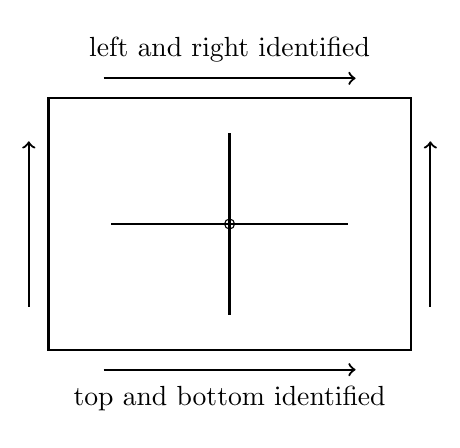
\begin{tikzpicture}[scale=1.0]
\draw[thick] (0,0) rectangle (4.6,3.2);

\draw[->,thick] (0.7,3.45)--(3.9,3.45);
\draw[->,thick] (0.7,-0.25)--(3.9,-0.25);

\draw[->,thick] (-0.25,0.55)--(-0.25,2.65);
\draw[->,thick] (4.85,0.55)--(4.85,2.65);

\draw[thick] (0.8,1.6)--(3.8,1.6);
\draw[thick] (2.3,0.45)--(2.3,2.75);

\draw (2.3,1.6) circle (1.8pt);

\draw (2.3,-0.62) node {top and bottom identified};
\draw (2.3,3.82) node {left and right identified};
\end{tikzpicture}
\caption{Một xuyến phẳng được dựng bằng cách đồng nhất các cạnh đối diện của một hình chữ nhật. Các cạnh không phải là biên; các điểm được ghép cặp chính là cùng một điểm của không gian thương.}
\label{fig:c03-flat-torus}
\end{figure}

\begin{classroomqa}
\audiencequestion{Vậy một vũ trụ có thể vừa phẳng vừa hữu hạn không?}
\lecturerresponse{Có. Độ phẳng là một phát biểu cục bộ về metric; tính hữu hạn có thể là một phát biểu toàn cục về tôpô. Một xuyến 3 chiều đủ lớn sẽ trông Euclid trong toàn bộ miền mà ta có thể quan sát, dù tổng thể tích của nó là hữu hạn. \lecturetimestamp{01:13:37--01:17:59}}
\end{classroomqa}

Bức tranh phủ phổ quát làm cho hệ quả quan sát được trở nên rõ ràng. Thay vì đồng nhất các cạnh, hãy lát một mặt phẳng Euclid vô hạn bằng các bản sao của hình chữ nhật cơ bản. Một vật thể duy nhất trong xuyến xuất hiện một lần trong mỗi bản sao. Trong 3 chiều, các bản sao tạo thành một mạng tuần hoàn kiểu tinh thể.

\begin{classroomqa}
\audiencequestion{Liệu ta có thể sống trong một vũ trụ dạng xuyến mà không nhận ra điều đó không?}
\lecturerresponse{Có, nếu ô cơ sở lớn hơn miền mà từ đó ánh sáng đã tới được chỗ ta. Nếu nó đủ nhỏ, ánh sáng có thể đi qua các phép đồng nhất và ta sẽ thấy các ảnh lặp của cùng những thiên hà, thậm chí có thể cả những cái nhìn lặp lại về chính vùng lân cận của chúng ta, theo các hướng khác nhau. Hình học cục bộ trong cả hai trường hợp vẫn phẳng. \lecturetimestamp{01:18:16--01:22:04}}
\end{classroomqa}

\begin{classroomqa}
\audiencequestion{Vì sao cầu dừng lại ở điểm đối cực của nó còn xuyến thì lặp lại?}
\lecturerresponse{Trên cầu, lớp vỏ bao quanh thực sự co về 0 tại \(r=\pi\); mọi hướng xuyên tâm đều gặp nhau ở điểm đối cực. Trên xuyến, cạnh của ô chữ nhật được chọn không bao giờ co lại. Nó được đồng nhất với một cạnh đối diện lớn bằng nó, nên đi qua đó chỉ là tiếp tục cùng một không gian trong một mô tả tọa độ tuần hoàn. \lecturetimestamp{01:22:06--01:23:02}}
\end{classroomqa}

\section{Từ không gian đến không-thời gian}

Giờ ta có thể đưa thời gian trở lại. Trong hệ đơn vị với tốc độ ánh sáng \(c=1\), metric Minkowski là
\begin{equation}
ds^2 = -dt^2 + dx^2 + dy^2 + dz^2.
\label{eq:c03-minkowski}
\end{equation}
Quy ước dấu là một lựa chọn; điều quan trọng là hạng thời gian có dấu ngược với các hạng không gian. Một tia sáng đi theo một quỹ đạo null,
\begin{equation}
ds^2 = 0.
\end{equation}
Đối với chuyển động chỉ dọc theo \(x\),
\begin{equation}
-dt^2 + dx^2 = 0
\qquad\Rightarrow\qquad
dx = \pm dt.
\label{eq:c03-null-flat}
\end{equation}
Hai dấu mô tả ánh sáng chuyển động sang trái hoặc sang phải với tốc độ đơn vị.

Đối với vũ trụ học, ta giữ hạng thời gian riêng \(-dt^2\), thay phần không gian Euclid bằng một metric không gian đồng nhất, và cho phép thang tổng thể của nó biến thiên theo thời gian. Ta ký hiệu thừa số tỉ lệ này là \(a(t)\). Bây giờ nó là một hàm động lực học chứ không phải bán kính cố định \(R_c\) được dùng trong phép so sánh tĩnh.

Lấy một ví dụ \(2+1\) chiều có thể hình dung được,
\begin{equation}
ds^2 = -dt^2 + a(t)^2 d\Omega_2^2.
\label{eq:c03-two-plus-one}
\end{equation}
Ở mỗi \(t\) cố định, không gian là một cầu \(2\)-chiều bán kính \(a(t)\). Xếp chồng các cầu này theo thời gian ta được không-thời gian. Phép dựng quen thuộc trong \(3+1\) chiều là
\begin{equation}
ds^2 = -dt^2 + a(t)^2 d\Sigma^2,
\label{eq:c03-frw-general}
\end{equation}
trong đó \(d\Sigma^2\) là một metric không gian đơn vị không phụ thuộc thời gian. Ba trường hợp đơn liên là
\begin{align}
\text{flat:}\quad
ds^2&=-dt^2+a(t)^2\left(dx^2+dy^2+dz^2\right),\label{eq:c03-frw-flat}\\
\text{spherical:}\quad
ds^2&=-dt^2+a(t)^2d\Omega_3^2,\label{eq:c03-frw-spherical}\\
\text{hyperbolic:}\quad
ds^2&=-dt^2+a(t)^2dh_3^2.\label{eq:c03-frw-hyperbolic}
\end{align}
Tỉ lệ tương đối của các tọa độ đồng chuyển động được giữ cố định trong khi \(a(t)\) thay đổi. Trong các chuẩn hóa cầu và hyperbol, \(a(t)\) cũng là bán kính độ cong tức thời. Trong trường hợp phẳng, chuẩn hóa tuyệt đối của nó có thể được hấp thụ vào các tọa độ đồng chuyển động.

Định luật Hubble suy ra được trước khi ta áp đặt bất kỳ phương trình trường hấp dẫn nào. Xét hai điểm đồng chuyển động gần nhau có độ tách tọa độ cố định \(\chi\). Độ tách vật lý của chúng là
\begin{equation}
D(t)=a(t)\chi.
\label{eq:c03-comoving-distance}
\end{equation}
Lấy đạo hàm với \(\chi\) cố định, ta được
\begin{equation}
V=\dot D=\dot a(t)\chi.
\end{equation}
Khử \(\chi\),
\begin{equation}
V = \frac{\dot a}{a} D.
\label{eq:c03-hubble-law}
\end{equation}
Do đó
\begin{equation}
H = \frac{\dot a}{a}.
\label{eq:c03-hubble-parameter}
\end{equation}
Đây là một đồng nhất thức động học cho sự giãn nở hoặc co lại đồng nhất. Nó đúng cho cả ba hình học không gian: \(\dot a>0\) cho sự lùi ra xa, còn \(\dot a<0\) cho sự tiến lại gần.

Chỉ riêng hình học không xác định \(a(t)\). Những hàm như
\begin{equation}
a(t)\propto t^{2/3},
\qquad
a(t)\propto t^{1/2},
\qquad
a(t)\propto e^{Ht}
\end{equation}
đều phù hợp với ansatz metric đồng nhất nhưng mô tả các thành phần vật chất và năng lượng vũ trụ khác nhau. Thuyết tương đối rộng cung cấp phương trình động lực học để chọn giữa chúng. Phương trình Friedmann thu được cũng sẽ liên hệ các trường hợp phẳng, cầu và hyperbol với những khả năng năng lượng bằng 0, âm và dương của vũ trụ học Newton đã được phát triển trước đó.

\begin{classroomqa}
\audiencequestion{Liệu hình học và sự tiến hóa vũ trụ có thể phức tạp hơn nhiều so với các mô hình này không?}
\lecturerresponse{Chắc chắn có. Tính đồng nhất và đẳng hướng là những giả thiết mang tính hạn chế, được chọn vì chúng tự nhiên, thành công về mặt quan sát trên các thang lớn, và xử lý được về mặt toán học. Tồn tại nhiều hình học và tiến hóa phức tạp hơn. Một câu hỏi động lực học quan trọng là liệu những lớp rộng của các mô hình ban đầu không đều có tiến hóa về một trong những dạng đồng nhất đơn giản này hay không. \lecturetimestamp{01:36:00--01:36:50}}
\end{classroomqa}

\begin{classroomqa}
\audiencequestion{Cầu \(3\)-chiều có phải là biên của một vật thể 4 chiều không?}
\lecturerresponse{Nó có thể được biểu diễn như vậy dưới dạng một phép nhúng, nhưng không gian vũ trụ học chính là bản thân cầu \(3\)-chiều ấy. Nó có 3 chiều nội tại và không có biên. Hình dung Euclid 4 chiều chỉ là một khung phụ trợ tùy chọn; phương trình~\eqref{eq:c03-three-sphere} đã xác định đầy đủ hình học. \lecturetimestamp{01:36:55--01:37:59}}
\end{classroomqa}

\begin{classroomqa}
\audiencequestion{Độ sáng có phải là cách duy nhất để thu được khoảng cách cần cho phép kiểm tra độ cong không?}
\lecturerresponse{Không. Các vạch phổ cho phép xác định độ dịch đỏ, các bậc thang khoảng cách ở gần hiệu chuẩn quan hệ Hubble, và các siêu tân tinh cung cấp những độ sáng gần chuẩn. Những phương pháp này được đối chiếu chéo chứ không được tin dùng một cách cô lập. Ngay cả định luật độ sáng nghịch đảo bình phương cũng phụ thuộc vào hình học, vì diện tích của một mặt sóng ánh sáng được quyết định bởi \(r^2\), \(\sin^2r\), hoặc \(\sinh^2r\). Chính sự phù hợp của nhiều đại lượng quan sát mới hậu thuẫn cho tính gần phẳng. \lecturetimestamp{01:38:00--01:41:07}}
\end{classroomqa}

\section{Những điều cần ghi nhớ}

Hình học của một vũ trụ đồng nhất có thể được đọc ra từ sự lớn dần của các lớp vỏ cầu quanh bất kỳ người quan sát nào:
\begin{equation}
f(r)=
\begin{cases}
r, & \text{flat space},\\
\sin r, & \text{positive curvature},\\
\sinh r, & \text{negative curvature}.
\end{cases}
\end{equation}
Metric không gian là \(dr^2+f(r)^2d\Omega_{n-1}^2\). Chính hàm ấy chi phối kích thước góc và số lượng vật thể có trên một lớp vỏ, nên độ cong có ý nghĩa quan sát trực tiếp. Một bán kính độ cong lớn che giấu những khác biệt này ở địa phương, và một phép đồng nhất kiểu xuyến cho thấy độ cong cục bộ tự nó không quyết định kích thước toàn cục hay tôpô.

Việc thêm \(-dt^2\) và thừa số chung \(a(t)^2\) biến bất kỳ một trong ba metric không gian đồng nhất nào thành một không-thời gian vũ trụ học. Điều đó lập tức cho \(V=HD\) với \(H=\dot a/a\), nhưng vẫn để \(a(t)\) chưa được xác định. Vì thế, bước tiếp theo không phải là một bài tập hình học khác. Đó là bài toán động lực học: dùng các phương trình Einstein để xác định vật chất, bức xạ, độ cong và các dạng năng lượng khác làm cho thừa số tỉ lệ tiến hóa như thế nào.
